\documentclass{beamer}
\usetheme{Boadilla}
\usecolortheme{sidebartab}
\beamertemplatenavigationsymbolsempty
\setbeamertemplate{footline}[frame number]
\usepackage{hyperref} 
\usepackage{graphicx}
\usepackage{color}
\usepackage{booktabs}
\usepackage{listings}
\usepackage{soul}
\usepackage{tikz}
\usepackage[utf8]{inputenc}
\usepackage{CJKutf8}
\usetikzlibrary{shapes.geometric}

\definecolor{gray}{rgb}{0.4,0.4,0.4}
\definecolor{darkblue}{rgb}{0.0,0.0,0.6}
\definecolor{cyan}{rgb}{0.0,0.6,0.6}
\definecolor{lightgray}{gray}{0.8}

\lstset{
	basicstyle=\ttfamily,
	columns=fullflexible,
	showstringspaces=false,
	commentstyle=\color{gray}\upshape
}

\makeatletter
\newcommand\SoulColor{%
	\let\set@color\beamerorig@set@color
	\let\reset@color\beamerorig@reset@color}
\makeatother

\lstset{language=XML}

\title{Ontologien mit RDF Schema}
\author{Markus Stocker}
\date{11. Juni 2018}

\begin{document}

\maketitle

\begin{frame}{Rekapitulation}
	
	\begin{itemize}
		\item Was ist RDFS? Wofür verwendet man die Sprache?
		\item Was ist eine Klasse?
		\item Was ist \texttt{rdfs:subClassOf}?
		\item Was ermöglicht \texttt{rdfs:range}?
	\end{itemize}
	
\end{frame}

\begin{frame}{Übersicht}
	
	\begin{itemize}
		\item Was ist Ontologie?
		\item Bestandteile und Aufbau
		\item Ontologien mit RDFS
		\item Ontologien entwickeln
		\item Prot{\'e}g{\'e}
	\end{itemize}
	
\end{frame}

\begin{frame}{Was ist Ontologie?}
	
	\begin{itemize}
		\item Eine Disziplin der Philosphie
		\item Die Lehre vom Sein
		\item Befasst sich mit den Grundstrukturen der Wirklichkeit
		\item Die fundamentalen Klassen und Beziehungen existierender Dinge 
		\item Aristoteles 10 Kategorien: Substanz, Quantität, Relation, ...
	\end{itemize}
	
\end{frame}

\begin{frame}{Ontologie in der Informatik}
	
	\begin{itemize}
		\item Teil der Wissensrepräsentation im Gebiet Künstliche Intelligenz
		\item Beschreibung von ``Wissen'' über eine Domäne
		\item Begriffe und Beziehungen eines Gegenstandsbereiches
		\item Beispiel: Erdähnliche und Gas Planeten mit Satelliten
		\item Eine maschinenverarbeitbare (formale) Beschreibung 
		\item Beispiel: \texttt{TerrestrialPlanet rdfs:subClassOf Planet}
	\end{itemize}
	
\end{frame}

\begin{frame}{Ontologie in der Informatik}
	
	\begin{itemize}
		\item Konsensbildung zwischen mehreren Parteien (z.B. in Projekte)
		\item Dienen dem Austausch von Wissen zwischen Anwendungen
		\item Interoperabilität verbessern
	\end{itemize}
	
\end{frame}

\begin{frame}{Bestandteile einer Ontologie}
	
	\begin{itemize}
		\item Klassen (\emph{concepts}, \emph{classes})
		\begin{itemize}
			\item Mengen der Dinge mit gleichen Eigenschaften
			\item Auch als Begriffe bezeichnet
			\item Beispiel: Die Menge der Planeten
		\end{itemize}
		\item Relationen (\emph{relations}, \emph{properties})
		\begin{itemize}
			\item Dienen der Beschreibung von Eigenschaften
			\item Beziehungen zwischen Klassen und deren Instanzen
			\item Beispiel: Die Eigenschaft Radius, Beziehung zwischen Planet und Wert
		\end{itemize}
		\item Instanzen (\emph{instances}, \emph{individuals})
		\begin{itemize}
			\item Elemente einer oder mehrerer Klassen
			\item Auch als Objekte bezeichnet
			\item Beispiel: Der Planet Erde als Instanz der Klasse der Planeten
		\end{itemize}
	\end{itemize}
	
\end{frame}

\begin{frame}[fragile]{Aufbau einer Ontologie}

	\begin{itemize}
		\item Schema (\emph{terminological box}): Vokabular, Klassen und Relationen
		\item Inhalt (\emph{assertional box}): Instanzen/Individuum, Aussagen, Daten 
		\item Dabei verwenden Inhalte das Schema
		\item Beispiel
	\end{itemize}	
	
    \begin{center}
    	\begin{tabular}{c}
    		\begin{lstlisting}
ex:Planet rdfs:subClassOf rdfs:Class
ex:earth rdf:type ex:Planet
    		\end{lstlisting}
    	\end{tabular}
    \end{center}
    
	\begin{itemize}
		\item Das erste Tripel ist Schema
		\item Das zweite Tripel ist Inhalt
		\item \texttt{ex:Planet} ist eine Klasse
		\item \texttt{ex:earth} is eine Instanz (Individuum)
	\end{itemize}	
	
\end{frame}

\begin{frame}[fragile]{Aufbau einer Ontologie: Schema}
	
	\begin{itemize}
		\item Das Schema besteht aus Axiome
		\item Diese gelten als wahr
		\item Dienen zur Repräsentation von abstraktem Wissen
		\item Beispiele
	\end{itemize}	
	
	\begin{center}
		\begin{tabular}{c}
			\begin{lstlisting}
ex:TerrestrialPlanet rdfs:subClassOf ex:Planet
ex:radius rdfs:domain ex:Planet
			\end{lstlisting}
		\end{tabular}
	\end{center}	
	
\end{frame}

\begin{frame}[fragile]{Aufbau einer Ontologie: Inhalte}
	
	\begin{itemize}
		\item Die Inhalte bestehen aus Aussagen
		\item Dienen zur Repräsentation von konkretem Wissen
		\item Beispiele
	\end{itemize}	
	
	\begin{center}
		\begin{tabular}{c}
			\begin{lstlisting}
ex:earth ex:radius "6371"
ex:earth rdf:type ex:Planet
			\end{lstlisting}
		\end{tabular}
	\end{center}	
	
\end{frame}

\begin{frame}{Ontologien mit RDFS}
	
	\begin{itemize}
		\item RDFS ist eine Sprache mittels der man Ontologien erstellen kann
		\item RDFS Dokument ist eine Spezifikation von Wissen über eine Domäne
		\item Wobei die Spezifikation maschinenverarbeitbar ist
		\item Die wichtigsten Bestandteile der Sprache haben wir bereits gesehen
		\item Insb. \texttt{rdfs:Class}, \texttt{rdfs:subClassOf}, \texttt{rdfs:subPropertyOf}
	\end{itemize}
	
\end{frame}

\begin{frame}{Ontologien Entwickeln}
	
	\begin{itemize}
		\item Ontologien entwickeln (\emph{ontology engineering}) ist eine eigene Disziplin
		\item Über einfache Beispiele hinaus, ist die Aufgabe generell komplex
		\item Schwierigkeit nicht primär im Erlernen von Technologie (z.B. RDFS)
		\item Schwieriger ist Wissen aus Köpfen in Dokumente zu formalisieren
	\end{itemize}
	
\end{frame}

\begin{frame}{Ontologien Entwickeln}
	
	\begin{itemize}
		\item Der zweck der Ontologie spielt eine wichtige Rolle
		\item Oft bestimmt der Zweck welche Aspekte man formalisiert
		\item Entwicklung von Ontologien also strukturiert angehen
		\item Insbesondere auch Anforderungsanalyse durchführen
		\item Ähnlich wie bei der Entwicklung von Software
	\end{itemize}
	
\end{frame}

\begin{frame}{Ontologien Entwickeln}
	
	\begin{itemize}
		\item Zuerst schauen ob es bereits eine entsprechende \textit{}Ontologie gibt
		\item Die wiederverwendet werden kann, auch nur Teilweise
		\item Eventuell gibt es eine übergeordnete Ontologie
		\item Welche abstrakteres Wissen formalisiert
		\item Auf einer solchen Aufbauen ist oft hilfreich
	\end{itemize}
	
\end{frame}

\begin{frame}{Anforderungsanalyse}
	
	\begin{itemize}
		\item Benötigt die Anwendung eine Ontologie, semantische Repräsentation?
		\item Oder genügt eine klassische Datenbank (u.U. bereits vorhanden)?
		\item Ist die Toolunterstützung adäquat für mein Projekt?
		\item Wie sind die Tools lizensiert und wie ausgereift sind sie?
	\end{itemize}
	
\end{frame}

\begin{frame}{Anforderungsanalyse}
	
	\begin{itemize}
		\item Welche Domäne wird modelliert?
		\item Welche Aspekte müssen erfasst werden?
		\item Wie detalliert soll Wissen beschrieben werden?
		\item Welche Tätigkeiten soll die Ontologie unterstützen?
	\end{itemize}
	
\end{frame}

\begin{frame}{Ontologie Erstellen}
	
	\begin{itemize}
		\item Übersetzung von Wissen in eine maschinenlesbare Form
		\item Es gibt mehrere Arten von Quellen für Wissen
		\item Z.B. menschliche Köpfe, Bücher, Web, Datenbanken
		\item Einige Quellen eignen sich besser als andere für Formalisierung
	\end{itemize}
	
\end{frame}

\begin{frame}{Wissensquelle: Mensch}
	
	\begin{itemize}
		\item Experten halten viel Wissen in Köpfen
		\item Die meisten können Wissen aber nicht formalisieren
		\item Weil sie sich mit RDFS nicht auskennen
		\item Zusammenarbeit mit ``Wissensingenieure'' nötig
		\item Diese führen Interviews durch und erfassen Expertenwissen
		\item Experten können nicht immer dinge genau definieren
		\item In der Kommunikation können Misverständnisse entstehen
	\end{itemize}
	
\end{frame}

{
	\usebackgroundtemplate{ %
		\begin{tikzpicture}[remember picture, overlay]%
		\node at (current page.center) {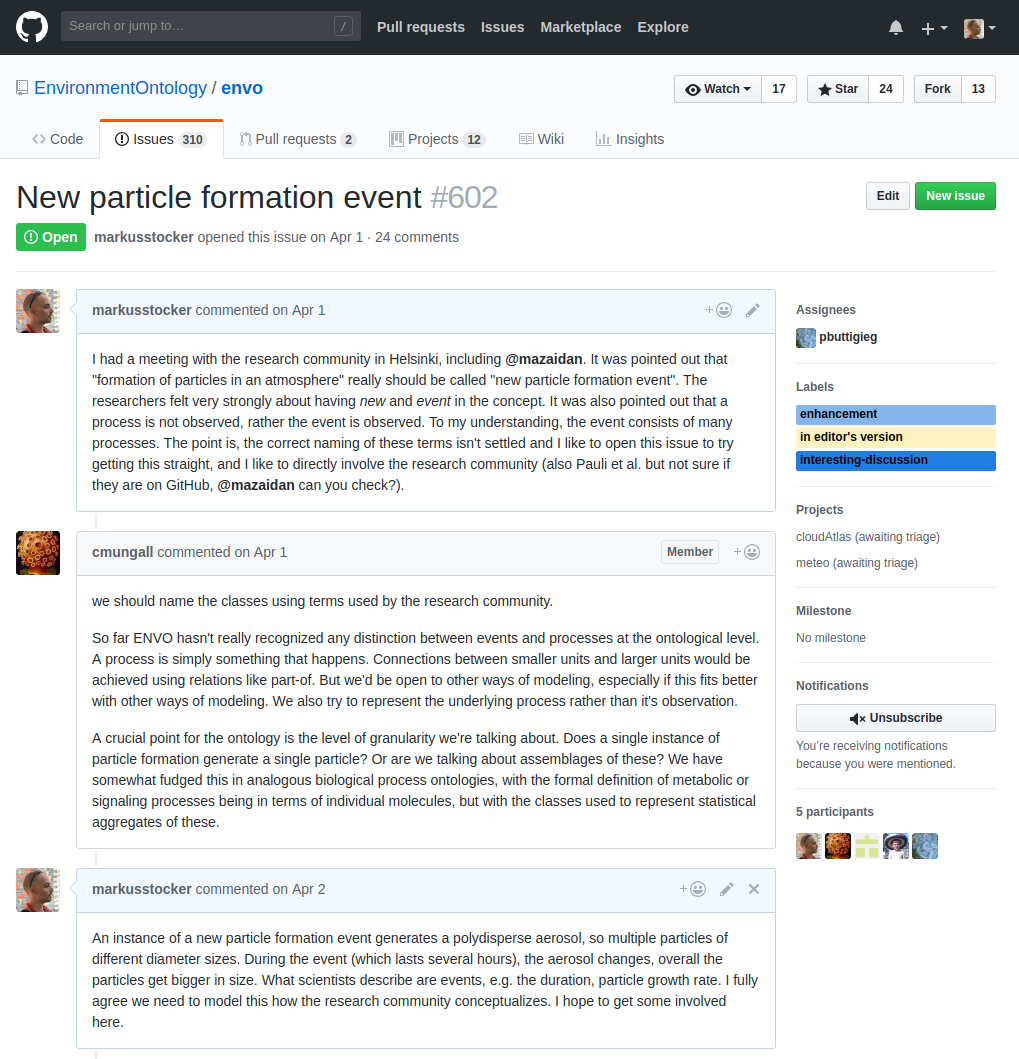
\includegraphics[height=\paperheight]{github-envo-npfe.png}};%
		\end{tikzpicture}%
	}%
	\setbeamertemplate{footline}[frame number]
	\begin{frame}[plain]

	\end{frame}
}


\begin{frame}{Wissensquelle: Bücher (Unstrukturiert)}
	
	\begin{itemize}
		\item Text ist einfach für Menschen zu verarbeiten
		\item Formales Wissen aus Text (automatisiert) zu extrahieren ist schwierig
		\item Natürliche Sprache ist oft mehrdeutig, kontextabhängig, usw.
		\item Der Prozess leidet meist unter Informationsverlust
		\item Obwohl hier viel geforscht wurde, sind Resultate eher bescheiden
	\end{itemize}
	
\end{frame}

\begin{frame}{Wissensquelle: Web (Semistrukturiert)}
	
	\begin{itemize}
		\item Gewisse Inhalte kommen Strukturiert daher
		\item Beispiel: Wikipedia Artikel enthalten auch strukturierte Information
		\item Solche Inhalte kann man einfacher formalisieren
		\item Struktur gibt es auch zwischen Inhalten
		\item Beispiel: Explizite Verlinkung zwischen Seiten
		\item Weist auf eine Verbundenheit hin, wobei die Art oft unklar bleibt
		\item Metadaten sind oft Strukturiert
		\item Beispiel: Exif in Bilder
		\item Bildinhalt unbekannt aber Zugang auf Dateiname/-grösse/-typ, Zeit
	\end{itemize}
	
\end{frame}

\begin{frame}{Wissensquelle: Datenbanken (Strukturiert)}
	
	\begin{itemize}
		\item Datenbankinhalte können meist nach RDF übersetzt werden
		\item Damit erhält man auf einfache Weise semantische Aussagen
		\item Schemainformation kann man zusätzlich verwenden
		\item Um terminologisches Wissen aufzubauen
		\item Andere Ontologien sind auch Quellen für bereits formalisiertes Wissen
	\end{itemize}
	
\end{frame}

\begin{frame}{Ontologien Bearbeiten: Prot{\'e}g{\'e}}
	
	\begin{itemize}
		\item Prot{\'e}g{\'e} ist ein Programm mit dem man Ontologien editieren kann
		\item Frei erhältlich unter https://protege.stanford.edu
		\item Als Lokalinstallation oder im Web verfügbar
		\item Web Version unter https://webprotege.stanford.edu/
		\item Wir benutzen Prot{\'e}g{\'e} um eine kleine Ontologie zu entwickeln
	\end{itemize}
	
\end{frame}

{
	\usebackgroundtemplate{ %
		\begin{tikzpicture}[remember picture, overlay]%
		\node at (current page.center) {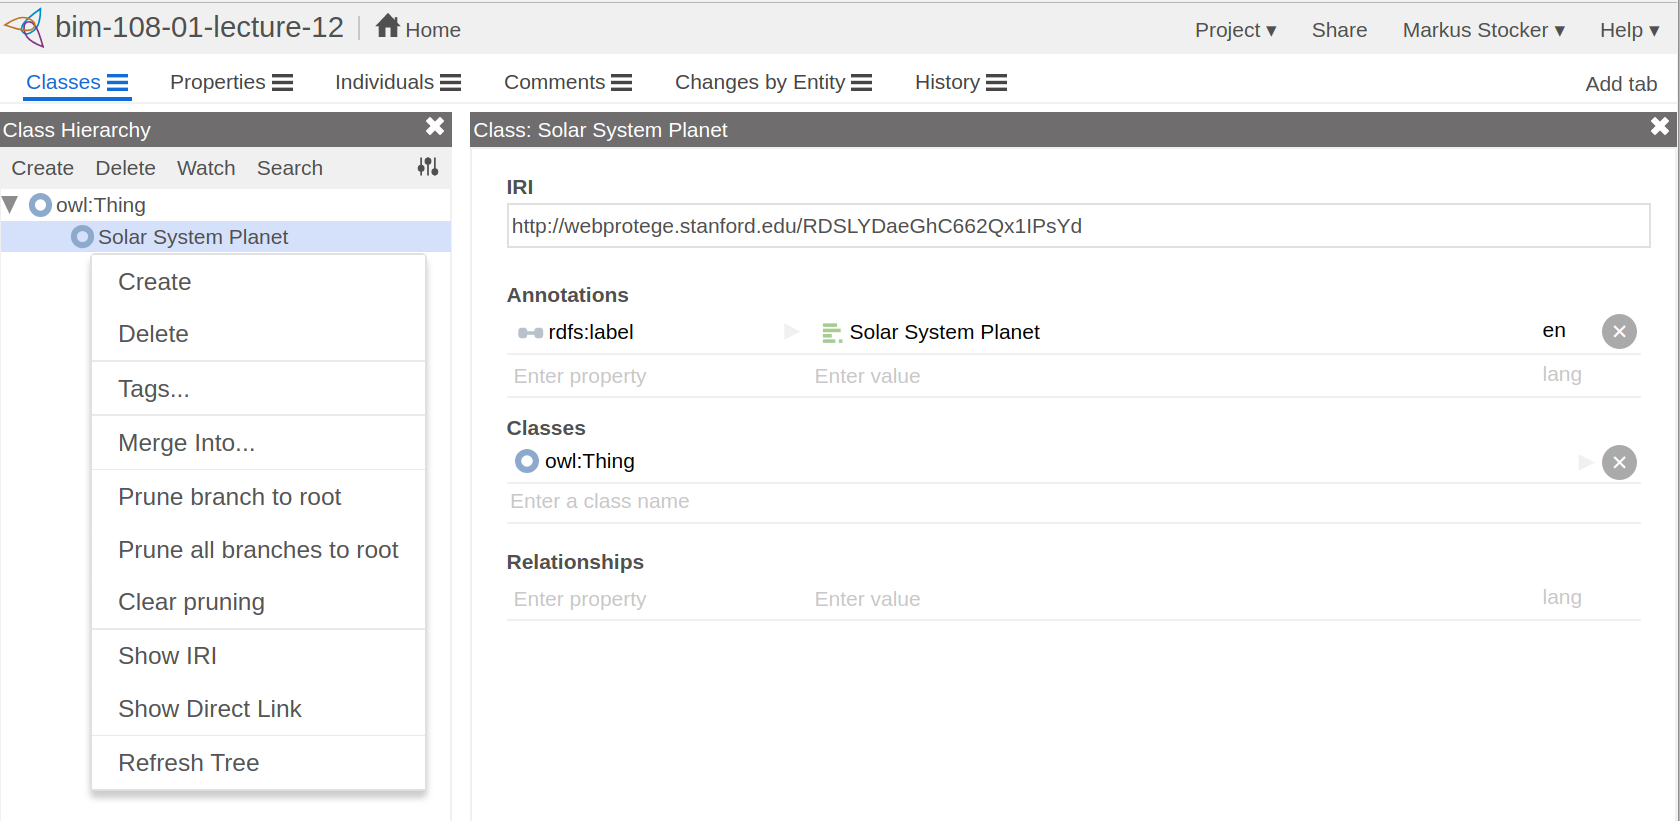
\includegraphics[width=\paperwidth]{webprotege-create-class.png}};%
		\end{tikzpicture}%
	}%
	\setbeamertemplate{footline}[frame number]
	\begin{frame}[plain]
		
	\end{frame}
}

{
	\usebackgroundtemplate{ %
		\begin{tikzpicture}[remember picture, overlay]%
		\node at (current page.center) {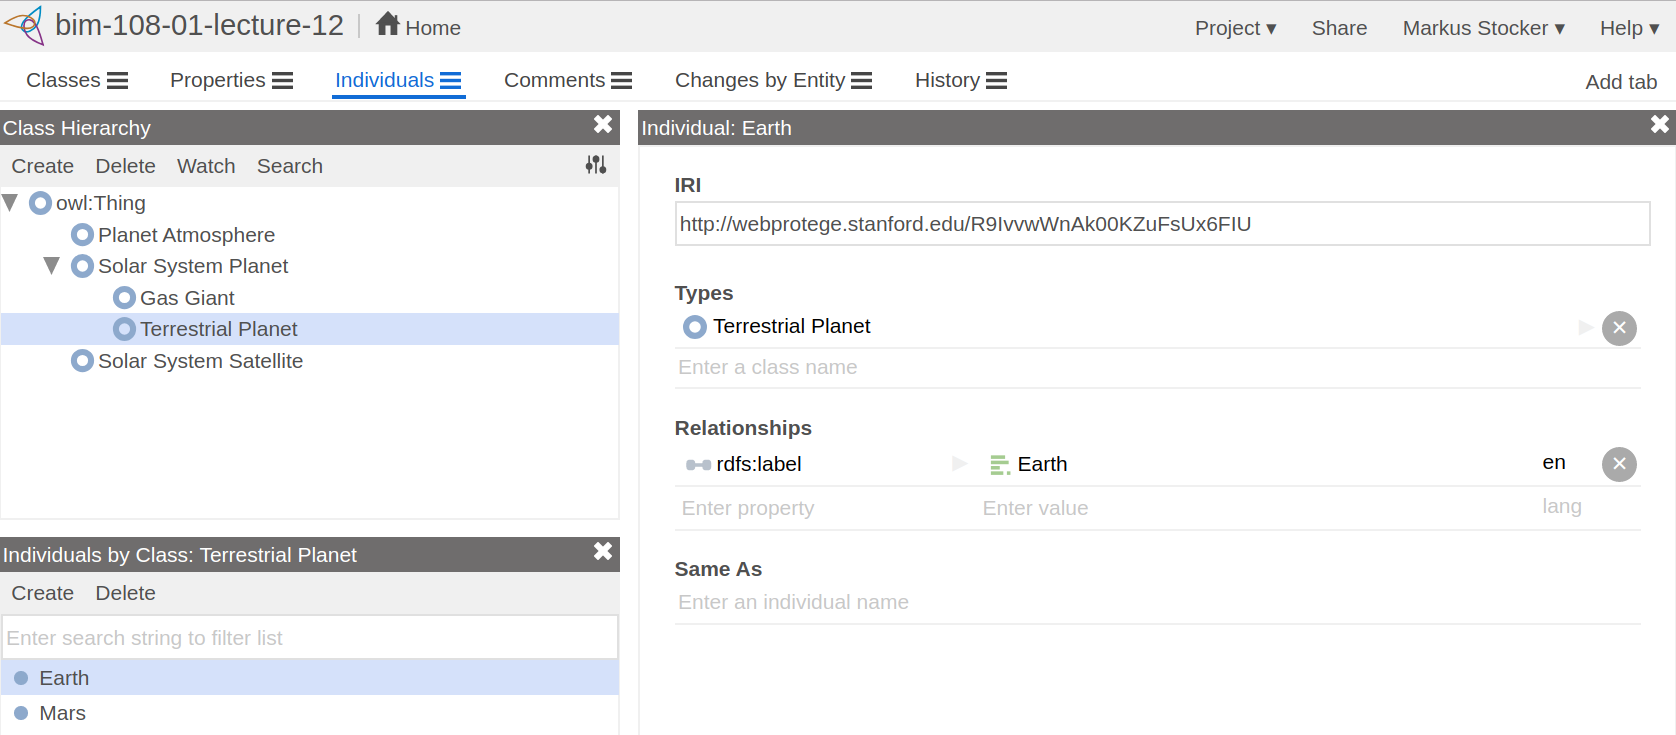
\includegraphics[width=\paperwidth]{webprotege-create-individual.png}};%
		\end{tikzpicture}%
	}%
	\setbeamertemplate{footline}[frame number]
	\begin{frame}[plain]
		
	\end{frame}
}

{
	\usebackgroundtemplate{ %
		\begin{tikzpicture}[remember picture, overlay]%
		\node at (current page.center) {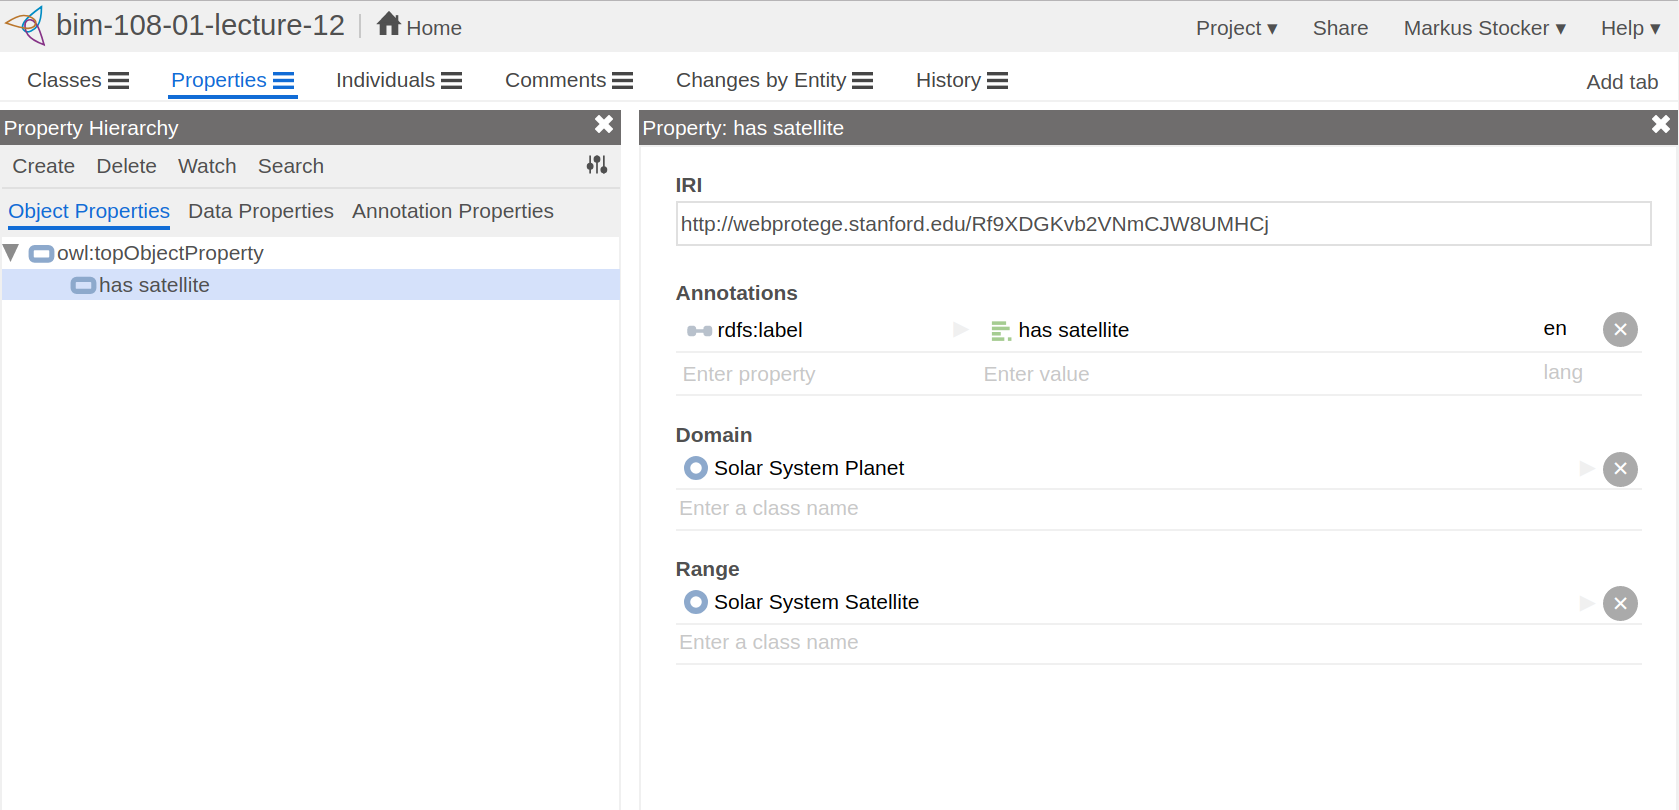
\includegraphics[width=\paperwidth]{webprotege-create-objectproperty.png}};%
		\end{tikzpicture}%
	}%
	\setbeamertemplate{footline}[frame number]
	\begin{frame}[plain]
		
	\end{frame}
}


{
	\usebackgroundtemplate{ %
		\begin{tikzpicture}[remember picture, overlay]%
		\node at (current page.center) {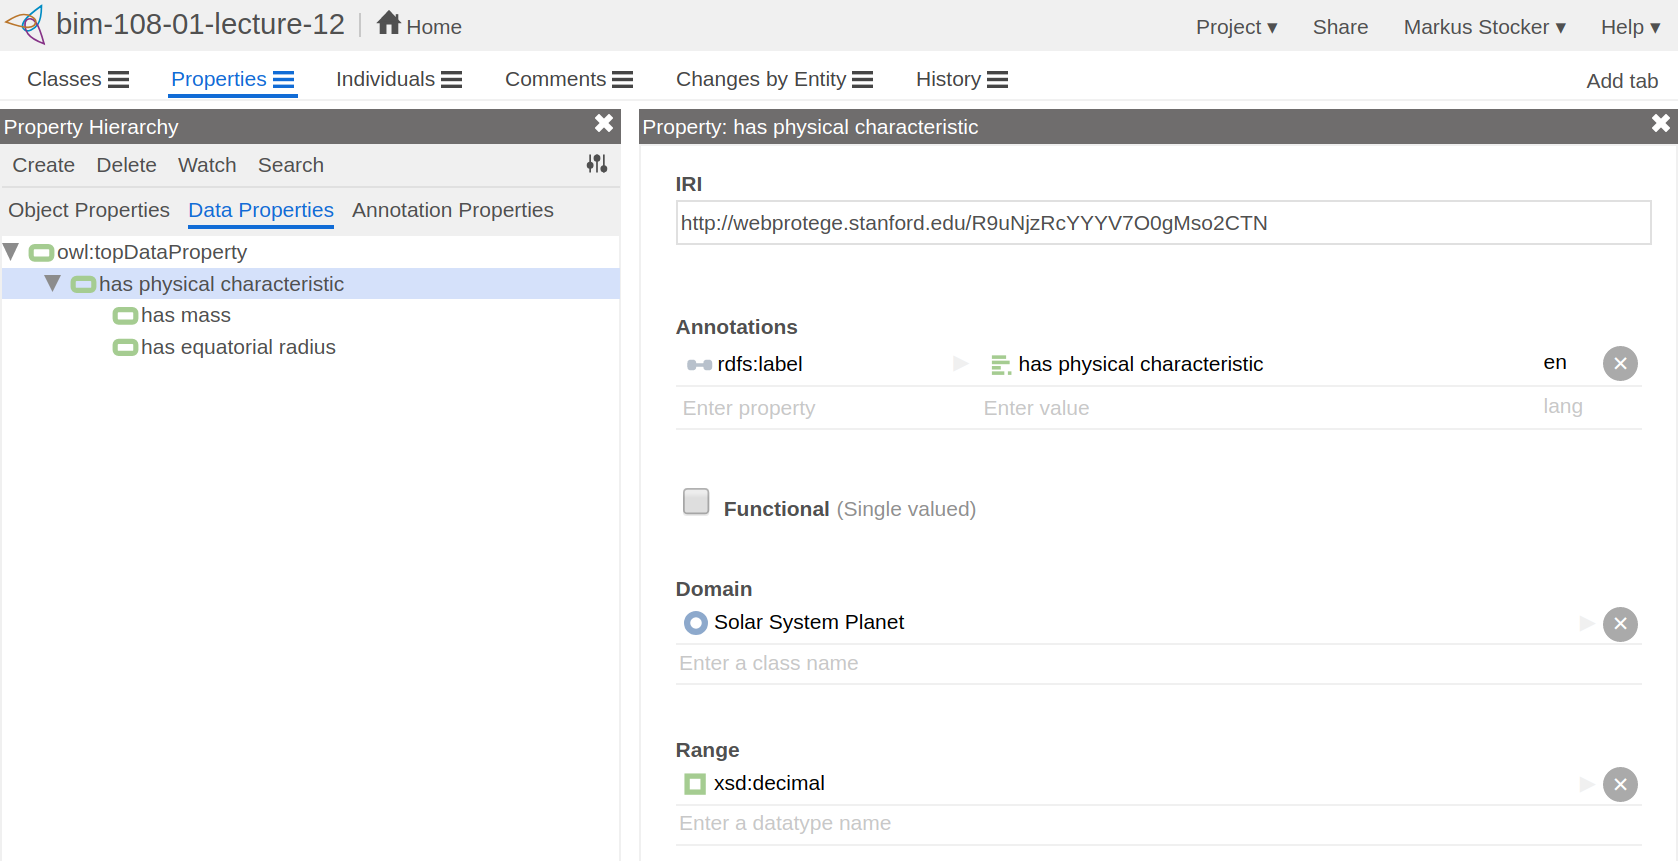
\includegraphics[width=\paperwidth]{webprotege-create-dataproperty.png}};%
		\end{tikzpicture}%
	}%
	\setbeamertemplate{footline}[frame number]
	\begin{frame}[plain]
		
	\end{frame}
}

{
	\usebackgroundtemplate{ %
		\begin{tikzpicture}[remember picture, overlay]%
		\node at (current page.center) {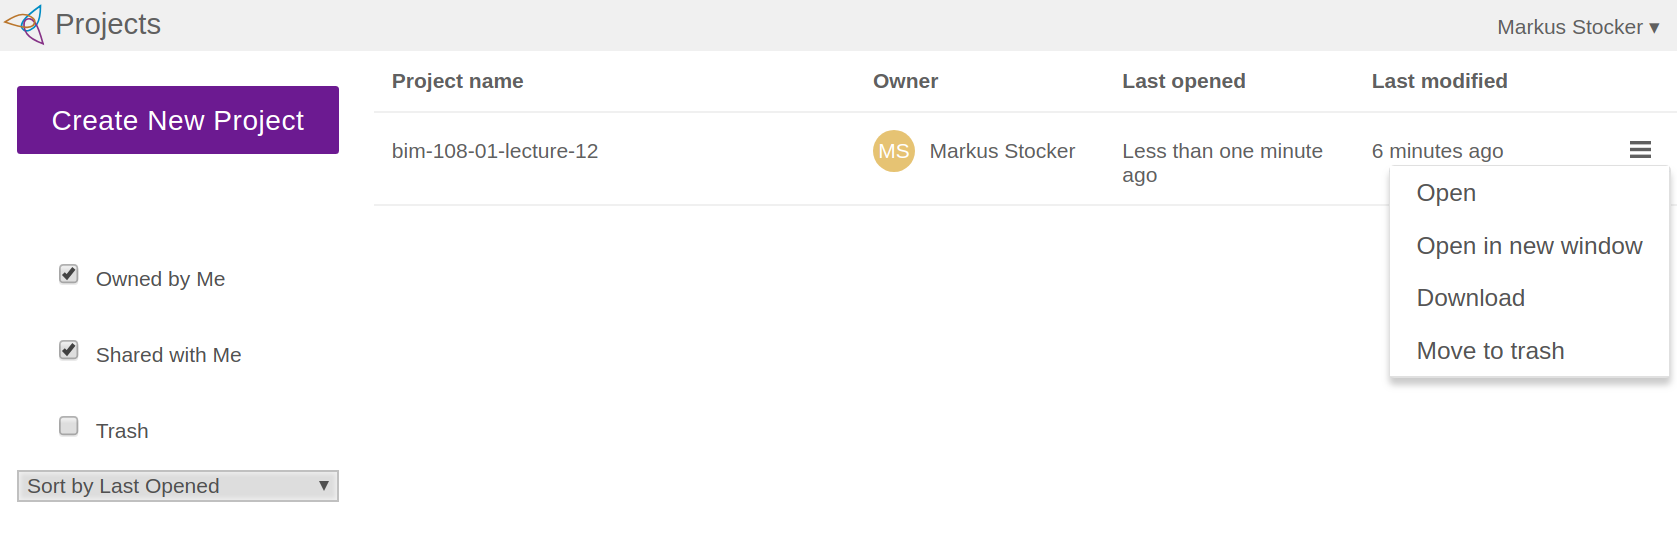
\includegraphics[width=\paperwidth]{webprotege-download.png}};%
		\end{tikzpicture}%
	}%
	\setbeamertemplate{footline}[frame number]
	\begin{frame}[plain]
		
	\end{frame}
}

\begin{frame}{Zusammenfassung}
	
	\begin{itemize}
		\item Mit Ontologien kann man Wissen formalisieren
		\item Mit RDFS können einfache Ontologien erstellt werden
		\item Die Sprache hat eine relativ kleine Expressivität
		\item Man kann nur ``einfaches Wissen'' ausdrücken
		\item Es gibt noch weitere ausdruckstärkere Sprachen (OWL) 
		\item Die Entwicklung von Ontologien ist generell komplex
		\item Die Aufgabe muss somit strukturiert angegangen werden
	\end{itemize}
	
\end{frame}

\end{document}